\documentclass{article}
%%%%%%%%%%%%%%%%%%%%%%%%%%%%% Define Article %%%%%%%%%%%%%%%%%%%%%%%%%%%%%%%%%%
%%%%%%%%%%%%%%%%%%%%%%%%%%%%%%%%%%%%%%%%%%%%%%%%%%%%%%%%%%%%%%%%%%%%%%%%%%%%%%%

%%%%%%%%%%%%%%%%%%%%%%%%%%%%% Using Packages %%%%%%%%%%%%%%%%%%%%%%%%%%%%%%%%%%
\usepackage{float}
\usepackage[letterpaper,portrait]{geometry}
\usepackage{graphicx}
\usepackage{anysize}
\usepackage{lipsum}
\usepackage{amsmath,amssymb,amsthm}
\usepackage[utf8]{inputenc}
\usepackage{multirow}
\usepackage{csquotes}
\usepackage[spanish]{babel}
\usepackage{apacite}
\usepackage{multicol}
\usepackage{parskip}
\usepackage{setspace}
\usepackage{empheq}
\usepackage{mdframed}
\usepackage{booktabs}
\usepackage{lipsum}
\usepackage{graphicx}
\usepackage{color}
\usepackage{psfrag}
\usepackage{pgfplots}
\usepackage{bm}
\usepackage{tocloft}
\usepackage{lscape}
\usepackage{adjustbox}
\setlength{\tabcolsep}{1.505625pt}
\renewcommand{\arraystretch}{1.2}
%%%%%%%%%%%%%%%%%%%%%%%%%%%%%%%%%%%%%%%%%%%%%%%%%%%%%%%%%%%%%%%%%%%%%%%%%%%%%%%

% Other Settings

%%%%%%%%%%%%%%%%%%%%%%%%%% Page Setting %%%%%%%%%%%%%%%%%%%%%%%%%%%%%%%%%%%%%%%
\geometry{letterpaper, margin=2.54cm}

%%%%%%%%%%%%%%%%%%%%%%%%%% Define some useful colors %%%%%%%%%%%%%%%%%%%%%%%%%%
\definecolor{ocre}{RGB}{243,102,25}
\definecolor{mygray}{RGB}{243,243,244}
\definecolor{deepGreen}{RGB}{26,111,0}
\definecolor{shallowGreen}{RGB}{235,255,255}
\definecolor{deepBlue}{RGB}{61,124,222}
\definecolor{shallowBlue}{RGB}{235,249,255}
%%%%%%%%%%%%%%%%%%%%%%%%%%%%%%%%%%%%%%%%%%%%%%%%%%%%%%%%%%%%%%%%%%%%%%%%%%%%%%%

%%%%%%%%%%%%%%%%%%%%%%%%%% Define an orangebox command %%%%%%%%%%%%%%%%%%%%%%%%
\newcommand\orangebox[1]{\fcolorbox{ocre}{mygray}{hspace{1em}#1hspace{1em}}}
%%%%%%%%%%%%%%%%%%%%%%%%%%%%%%%%%%%%%%%%%%%%%%%%%%%%%%%%%%%%%%%%%%%%%%%%%%%%%%%

%%%%%%%%%%%%%%%%%%%%%%%%%%%% English Environments %%%%%%%%%%%%%%%%%%%%%%%%%%%%%
\newtheoremstyle{mytheoremstyle}{3pt}{3pt}{\normalfont}{0cm}{\rmfamily\bfseries}{}{1em}{{\color{black}\thmname{#1}~\thmnumber{#2}}\thmnote{\,--\,#3}}
\newtheoremstyle{myproblemstyle}{3pt}{3pt}{\normalfont}{0cm}{\rmfamily\bfseries}{}{1em}{{\color{black}\thmname{#1}~\thmnumber{#2}}\thmnote{\,--\,#3}}
\theoremstyle{mytheoremstyle}
\newmdtheoremenv[linewidth=1pt,backgroundcolor=shallowGreen,linecolor=deepGreen,leftmargin=0pt,innerleftmargin=20pt,innerrightmargin=20pt,]{theorem}{Theorem}[section]
\theoremstyle{mytheoremstyle}
\newmdtheoremenv[linewidth=1pt,backgroundcolor=shallowBlue,linecolor=deepBlue,leftmargin=0pt,innerleftmargin=20pt,innerrightmargin=20pt,]{definition}{Definition}[section]
\theoremstyle{myproblemstyle}
\newmdtheoremenv[linecolor=black,leftmargin=0pt,innerleftmargin=10pt,innerrightmargin=10pt,]{problem}{Problem}[section]
%%%%%%%%%%%%%%%%%%%%%%%%%%%%%%%%%%%%%%%%%%%%%%%%%%%%%%%%%%%%%%%%%%%%%%%%%%%%%%%

%%%%%%%%%%%%%%%%%%%%%%%%%%%%%%% Plotting Settings %%%%%%%%%%%%%%%%%%%%%%%%%%%%%
\usepgfplotslibrary{colorbrewer}
\pgfplotsset{width=8cm,compat=1.9}
%%%%%%%%%%%%%%%%%%%%%%%%%%%%%%%%%%%%%%%%%%%%%%%%%%%%%%%%%%%%%%%%%%%%%%%%%%%%%%%

%%%%%%%%%%%%%%%%%%%%%%%%%%%%%%% Title & Author %%%%%%%%%%%%%%%%%%%%%%%%%%%%%%%%
\author{Gustavo Vergara}
%%%%%%%%%%%%%%%%%%%%%%%%%%%%%%%%%%%%%%%%%%%%%%%%%%%%%%%%%%%%%%%%%%%%%%%%%%%%%%%

\begin{document}
\pgfplotsset{compat=1.18}
\setstretch{2}

\begin{titlepage}
	\centering
	\vspace{2.5cm}
	{\scshape \Large TAREA 1 DE MÁQUINAS TÉRMICAS\par}
	\vspace{5cm}
	\textbf\large\scshape{\par}
	\vspace{0.5cm}
	{\Large Vergara Pareja Gustavo\par}
	\vspace{5cm}
	{\scshape\Large Bernardo J. Luján E. \par}
	\vspace{0.3cm}
	{\scshape\Large Máquinas Térmicas - G2IM \par}
	\vspace{0.3cm}
	{\scshape\Large Universidad de Córdoba\par}
	\vspace{0.3cm}
	{\Large 6 de Diciembre de 2024 \par}
\end{titlepage}
\tableofcontents
\newpage
    \section{Estequiometría y exceso de aire}
    Los reactivos dados en porcentaje molar fueron los siguientes:
    \begin{figure}[h!] % 'h' indica que LaTeX debe intentar colocar la figura aquí
        \centering
        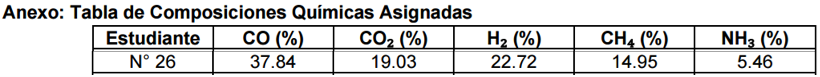
\includegraphics[width=1\textwidth]{comp.png} % Ajusta el ancho según necesites
        \caption{Composición del combustible}
        \label{fig:mi_imagen}
    \end{figure}

    Para este cálculo desarrollamos un balance de los reactivos y los productos. 
    
    \begin{equation}
        \label{EES Eqn:8}
        n_{CO} = 37.84\times 10^{-2}   \   \left[ \rm kmol \right] 
        \end{equation}
        {\color{blue} \rm}
        \begin{equation}
        \label{EES Eqn:9}
        n_{CO2} = 19.03\times 10^{-2}   \   \left[ \rm kmol \right] 
        \end{equation}
        {\color{blue} \rm}
        \begin{equation}
        \label{EES Eqn:10}
        n_{H2} = 22.72\times 10^{-2}   \   \left[ \rm kmol \right] 
        \end{equation}
        {\color{blue} \rm}
        \begin{equation}
        \label{EES Eqn:11}
        n_{CH4} = 14.95\times 10^{-2}   \   \left[ \rm kmol \right] 
        \end{equation}
        {\color{blue} \rm}
        \begin{equation}
        \label{EES Eqn:12}
        n_{NH3} = 5.46\times 10^{-2}   \   \left[ \rm kmol \right] 
        \end{equation}
        {\color{blue} \rm}
        \begin{equation}
        \label{EES Eqn:13}
        x = n_{CO} + n_{CO2} + n_{CH4} 
        \end{equation}
        \begin{equation}
        \label{EES Eqn:14}
        2\cdot y = 2\cdot n_{H2} +  \left( 4 \right) \cdot  \left( n_{CH4} \right)  +  \left( 3 \right) \cdot n_{NH3} 
        \end{equation}
        \begin{equation}
        \label{EES Eqn:15}
        z = 2 \cdot  3.76 \cdot  a_{s} + n_{NH3} 
        \end{equation}
        
        \vspace{0.10in}
        \noindent
        {\color{blue} \rm Para encontrar el aire teórico balanceamos el Oxígeno}
        \begin{equation}
        \label{EES Eqn:16}
        n_{CO} + 2\cdot n_{CO2} + a_{s}\cdot 2 = 2\cdot x + y 
        \end{equation}
       
        {\color{blue} \rm Así la ecuación balanceada queda:}
        \begin{equation}
            \scriptsize 0.3784\cdot CO + 0.1903 \cdot CO_2 + 0.2272\cdot H_2 + 0.1495 \cdot CH_4 + 0.0546 \cdot NH_3 + 0.6428\cdot (O_2 + 3.76\cdot N_2) \rightarrow 0.7182\cdot CO_2 + 0.6081 \cdot H_2O + 4.88808 \cdot N_2
        \end{equation}
        \it \textcolor{brown}{1.a Stoichiometric Air - Complete Comb} \\
${a_{s} =0.6428 \rm\ {\color{blue} \left[kmol\right]}}$ & 
\it \textcolor{brown}{} \\
Para calcular los productos de combustión con un exceso de aire, añadimos un factor \(\phi\) que incrementará en un 20\% el aire teórico.
\begin{equation}
    \label{EES Eqn:18}
    \phi = 1.2 
    \end{equation}
    \begin{equation}
    \label{EES Eqn:19}
    x_{e} = n_{CO} + n_{CO2} + n_{CH4} 
    \end{equation}
    \begin{equation}
    \label{EES Eqn:20}
    2\cdot y_{e} =  \left( 2 \right) \cdot n_{H2} +  \left( 4 \right) \cdot n_{CH4} +  \left( 3 \right) \cdot n_{NH3} 
    \end{equation}
    \begin{equation}
    \label{EES Eqn:21}
    2\cdot z_{e} = 2\cdot  3.76 \cdot  \phi \cdot  a_{s} + 1 \cdot  n_{NH3} 
    \end{equation}
    
    \vspace{0.10in}
    \noindent
    {\color{blue} \rm Para encontrar el Oxígeno en los productos balanceamos el oxígeno}
    \begin{equation}
    \label{EES Eqn:22}
    n_{CO} + 2\cdot n_{CO2} + a_{s}\cdot \phi\cdot 2 = 2\cdot x_{e} + y_{e} + 2\cdot w 
    \end{equation}
    \begin{equation}
    \label{EES Eqn:23}
    n_{product20} = x_{e} + y_{e} + z_{e} + w 
    \end{equation}
    \begin{equation}
    \label{EES Eqn:24}
    n_{CO2p} = x_{e} 
    \end{equation}
    \begin{equation}
    \label{EES Eqn:25}
    n_{H2O} = y_{e} 
    \end{equation}
    \begin{equation}
    \label{EES Eqn:26}
    n_{N2p} = z_{e} 
    \end{equation}
    \begin{equation}
    \label{EES Eqn:27}
    n_{O2p} = w 
    \end{equation}
    \it \textcolor{brown}{1.b Combustion Products with Excess Air} \\
    ${CO_2 =0.718200 \rm\ {\color{blue} \left[kmol\right]}}$ & 
    \it \textcolor{brown} \\
    ${H_2O =0.608100 \rm\ {\color{blue} \left[kmol\right]}}$ & 
    \it \textcolor{brown} \\
    ${N_2 =2.927388 \rm\ {\color{blue} \left[kmol\right]}}$ & 
    \it \textcolor{brown}\\
    ${O_2 =0.128550 \rm\ {\color{blue} \left[kmol\right]}}$ & 
    \it \textcolor{brown} \\
\newpage
\section{Temperatura de flama adiabática y calor de combustión (Qmax)}
Para calcular la flama adiabática a condiciones estándar, y con un exceso de aire del 20\%. Consideramos que no hay transferencia de calor, por lo tanto, Q=0.
Con los datos del inciso anterior, tenemos:
\begin{equation}
    \label{EES Eqn:28}
    n_{O2r} = \phi\cdot a_{s}\cdot 1 
    \end{equation}
    \begin{equation}
    \label{EES Eqn:29}
    n_{N2r} = \phi\cdot a_{s}\cdot 3.76 
    \end{equation}
    \begin{equation}
    \label{EES Eqn:30}
    T_{1} = \mbox{ConvertTemp}{ \left( C,\ K,\ 25 \right) } 
    \end{equation}
    \begin{equation}
    \label{EES Eqn:31}
    P_{1} = 1   \   \left[ \rm atm \right] \cdot  \rm { \left|101.325\ \frac {\rm{kPa}}{\rm{atm}}\right|} 
    \end{equation}
    {\color{blue} \rm}
    \begin{equation}
    \label{EES Eqn:32}
    P_{2} = P_{1} 
    \end{equation}
    \begin{equation}
    \label{EES Eqn:33}
    Q_{T} = W_{vc} + \sum_{e} (n \bar{h}_e)_P - \sum_{i} (n \bar{h}_i)_R
    \end{equation}
    \begin{equation}
        \label{EES Eqn:33}
        Q_{T} = 0 
        \end{equation}
    \begin{equation}
    \label{EES Eqn:34}
    \begin{align}
        Q_{T} &= n_{CO2p}\cdot h \left(\F{CO2},\mbox{\ T}=\V{T2}  \right)  + n_{H2O}\cdot h \left(\F{H2O},\mbox{\ T}=\V{T2}  \right)  + n_{N2p}\cdot h \left(\F{N2},\mbox{\ T}=\V{T2}  \right)  +  n_{O2p}\cdot h \left(\F{O2},\mbox{\ T}=\V{T2}  \right) \nonumber \\
        &\quad -  \left[ n_{CO}\cdot h \left(\F{CO},\mbox{\ T}=T_{1} \right)  + n_{CO2}\cdot h \left(\F{CO2},\mbox{\ T}=T_{1} \right)  + n_{H2}\cdot h \left(\F{H2},\mbox{\ T}=T_{1} \right)  + n_{CH4}\cdot h \left(\F{CH4},\mbox{\ T}=T_{1} \right) \right. \nonumber \\
        &\quad \left. + n_{NH3}\cdot h \left(\F{NH3},\mbox{\ T}=T_{1} \right)  + n_{O2r}\cdot h \left(\F{O2},\mbox{\ T}=T_{1} \right)  + n_{N2r}\cdot h \left(\F{N2},\mbox{\ T}=T_{1} \right) \right]
    \end{align}
    \end{equation}
    \it \textcolor{brown}{2.a Adiabatic Flame Temperature} \\
    ${\V{T2}  =2092.746437107 \rm\ {\color{blue} \left[K\right]}}$ & 
\newpage
    Para calcular el calor de combustión máximo, suponemos que entra y sale a condiciones estándar:
\begin{equation}
    \label{EES Eqn:35}
    T_{2} = T_{1} 
    \end{equation}
    \begin{equation}
    \label{EES Eqn:36}
    \begin{equation}
    \begin{split}
    Q_{max} = & \ n_{CO2p}\cdot h \left(\F{CO2},\mbox{\ T}=T_{2} \right)  + n_{H2O}\cdot h \left(\F{H2O},\mbox{\ T}=T_{2} \right)  + n_{N2p}\cdot h \left(\F{N2},\mbox{\ T}=T_{2} \right)  +  n_{O2p}\cdot h \left(\F{O2},\mbox{\ T}=T_{2} \right) \\
    & -  \left[ n_{CO}\cdot h \left(\F{CO},\mbox{\ T}=T_{1} \right)  + n_{CO2}\cdot h \left(\F{CO2},\mbox{\ T}=T_{1} \right)  + n_{H2}\cdot h \left(\F{H2},\mbox{\ T}=T_{1} \right)  + n_{CH4}\cdot h \left(\F{CH4},\mbox{\ T}=T_{1} \right) \right. \\
    & \left. + n_{NH3}\cdot h \left(\F{NH3},\mbox{\ T}=T_{1} \right)  + n_{O2r}\cdot h \left(\F{O2},\mbox{\ T}=T_{1} \right)  + n_{N2r}\cdot h \left(\F{N2},\mbox{\ T}=T_{1} \right) \right] 
    \end{split}
    \end{equation}

    \it \textcolor{brown}{2.b Heat Combustion Max - Standard Conditions} \\
${Q_{max} =-299283 \rm\ {\color{blue} \left[kJ\right]}}$ & 
\it \textcolor{brown}{Heat Combustion Max} \\

\newpage


\section{Poder calorífico y temperatura del punto de rocío}
        Para calcular el poder calorífico superior e inferior del combustible asignado, entonces:
        \begin{equation}
            \label{EES Eqn:1}
            M_{CO} = 28.013   \   \left[ \rm kg/kmol \right] 
            \end{equation}
            {\color{blue} \rm}
            \begin{equation}
            \label{EES Eqn:2}
            M_{CO2} =  \left( 44.01 \right)    \   \left[ \rm kg/kmol \right] 
            \end{equation}
            {\color{blue} \rm}
            \begin{equation}
            \label{EES Eqn:3}
            M_{H2} =  \left( 2.016 \right)    \   \left[ \rm kg/kmol \right] 
            \end{equation}
            {\color{blue} \rm}
            \begin{equation}
            \label{EES Eqn:4}
            M_{CH4} =  \left( 16.043 \right)    \   \left[ \rm kg/kmol \right] 
            \end{equation}
            {\color{blue} \rm}
            \begin{equation}
            \label{EES Eqn:5}
            M_{NH3} =  \left( 17.03 \right)    \   \left[ \rm kg/kmol \right] 
            \end{equation}
            {\color{blue} \rm}
            \begin{equation}
            \label{EES Eqn:6}
            M_{Air} = 39   \   \left[ \rm kg/kmol \right] 
            \end{equation}
            {\color{blue} \rm}
            \begin{equation}
            \label{EES Eqn:7}
            M_{H2O} = 18.02   \   \left[ \rm kg/kmol \right] 
            \end{equation}

        \begin{equation}
            \label{EES Eqn:37}
            M_{total} = M_{CO} + M_{CO2} + M_{H2} + M_{CH4} + M_{NH3} 
            \end{equation}
            \begin{equation}
            \label{EES Eqn:38}
            h_{c} = \V{abs}  \left( Q_{max} \right)  
            \end{equation}
            \begin{equation}
            \label{EES Eqn:39}
            \V{HHV}  = h_{c}/M_{total} 
            \end{equation}
            \begin{equation}
            \label{EES Eqn:40}
            y_{H2O} = n_{H2O}/n_{product} 
            \end{equation}
            \begin{equation}
            \label{EES Eqn:41}
            \V{LHV}  = \V{HHV}  - y_{H2O}\cdot \frac {h_{vaporization} \left(\F{Water},\mbox{\ P}=P_{1} \right) }{ M_{H2O} } 
            \end{equation}
            
            \it \textcolor{brown}{3.a HHV and LHV - Complete Comb} \\
${\V{HHV}  =2794 \rm\ {\color{blue} \left[kJ/kg\right]}}$ & 
\it \textcolor{brown}{} \\
${\V{LHV}  =2573 \rm\ {\color{blue} \left[kJ/kg\right]}}$ & 
\it \textcolor{brown}{} \\

Para determinar la temperatura de rocío, recalculamos la masa molar de los productos, cuando hay exceso de aire al 10\%
\begin{equation}
    \label{EES Eqn:42}
    \phi_{2} = 1.1 
    \end{equation}
    \begin{equation}
    \label{EES Eqn:43}
    x_{e2} = n_{CO} + n_{CO2} + n_{CH4} 
    \end{equation}
    \begin{equation}
    \label{EES Eqn:44}
    2\cdot y_{e2} =  \left( 2 \right) \cdot n_{H2} +  \left( 4 \right) \cdot n_{CH4} +  \left( 3 \right) \cdot n_{NH3} 
    \end{equation}
    \begin{equation}
    \label{EES Eqn:45}
    2\cdot z_{e2} = 2\cdot  3.76 \cdot  \phi_{2} \cdot  a_{s} + 1 \cdot  n_{NH3} 
    \end{equation}
    
    \vspace{0.10in}
    \noindent
    {\color{blue} \rm Para encontrar el exceso de Oxígeno balanceamos el Oxígeno}
    \begin{equation}
    \label{EES Eqn:46}
    n_{CO} + 2\cdot n_{CO2} + a_{s}\cdot \phi_{2}\cdot 2 = 2\cdot x_{e2} + y_{e2} + 2\cdot w_{22} 
    \end{equation}
    \begin{equation}
    \label{EES Eqn:47}
    n_{product10} = x_{e2} + y_{e2} + z_{e2} + w_{22} 
    \end{equation}
    \begin{equation}
    \label{EES Eqn:48}
    y_{H2O2} = n_{H2O}/n_{product10} 
    \end{equation}
    \begin{equation}
    \label{EES Eqn:49}
    P_{H2O} = y_{H2O2} \cdot  P_{1} 
    \end{equation}
    \begin{equation}
    \label{EES Eqn:50}
    T_{r} = T \left(\F{Water},\mbox{\ P}=P_{H2O},\mbox{\ x}=0 \right)  
    \end{equation}
    \hrulefill
    \\
   \it \textcolor{brown}{3.b Dew Point - Excess Air 10\%} \\
   ${T_{r} =327.3 \rm\ {\color{blue} \left[K\right]} \hspace{0.05in}\textcolor{brown}{\{54.14\left[C\right]\}}$ & 
   \it \textcolor{brown}{} \\
   \hrulefill

   \section{Conclusiones}

\subsection*{Plot Window 1:\;ExcessAir\;vs\;T[1]\;vs\;FlameT}
{\centerline{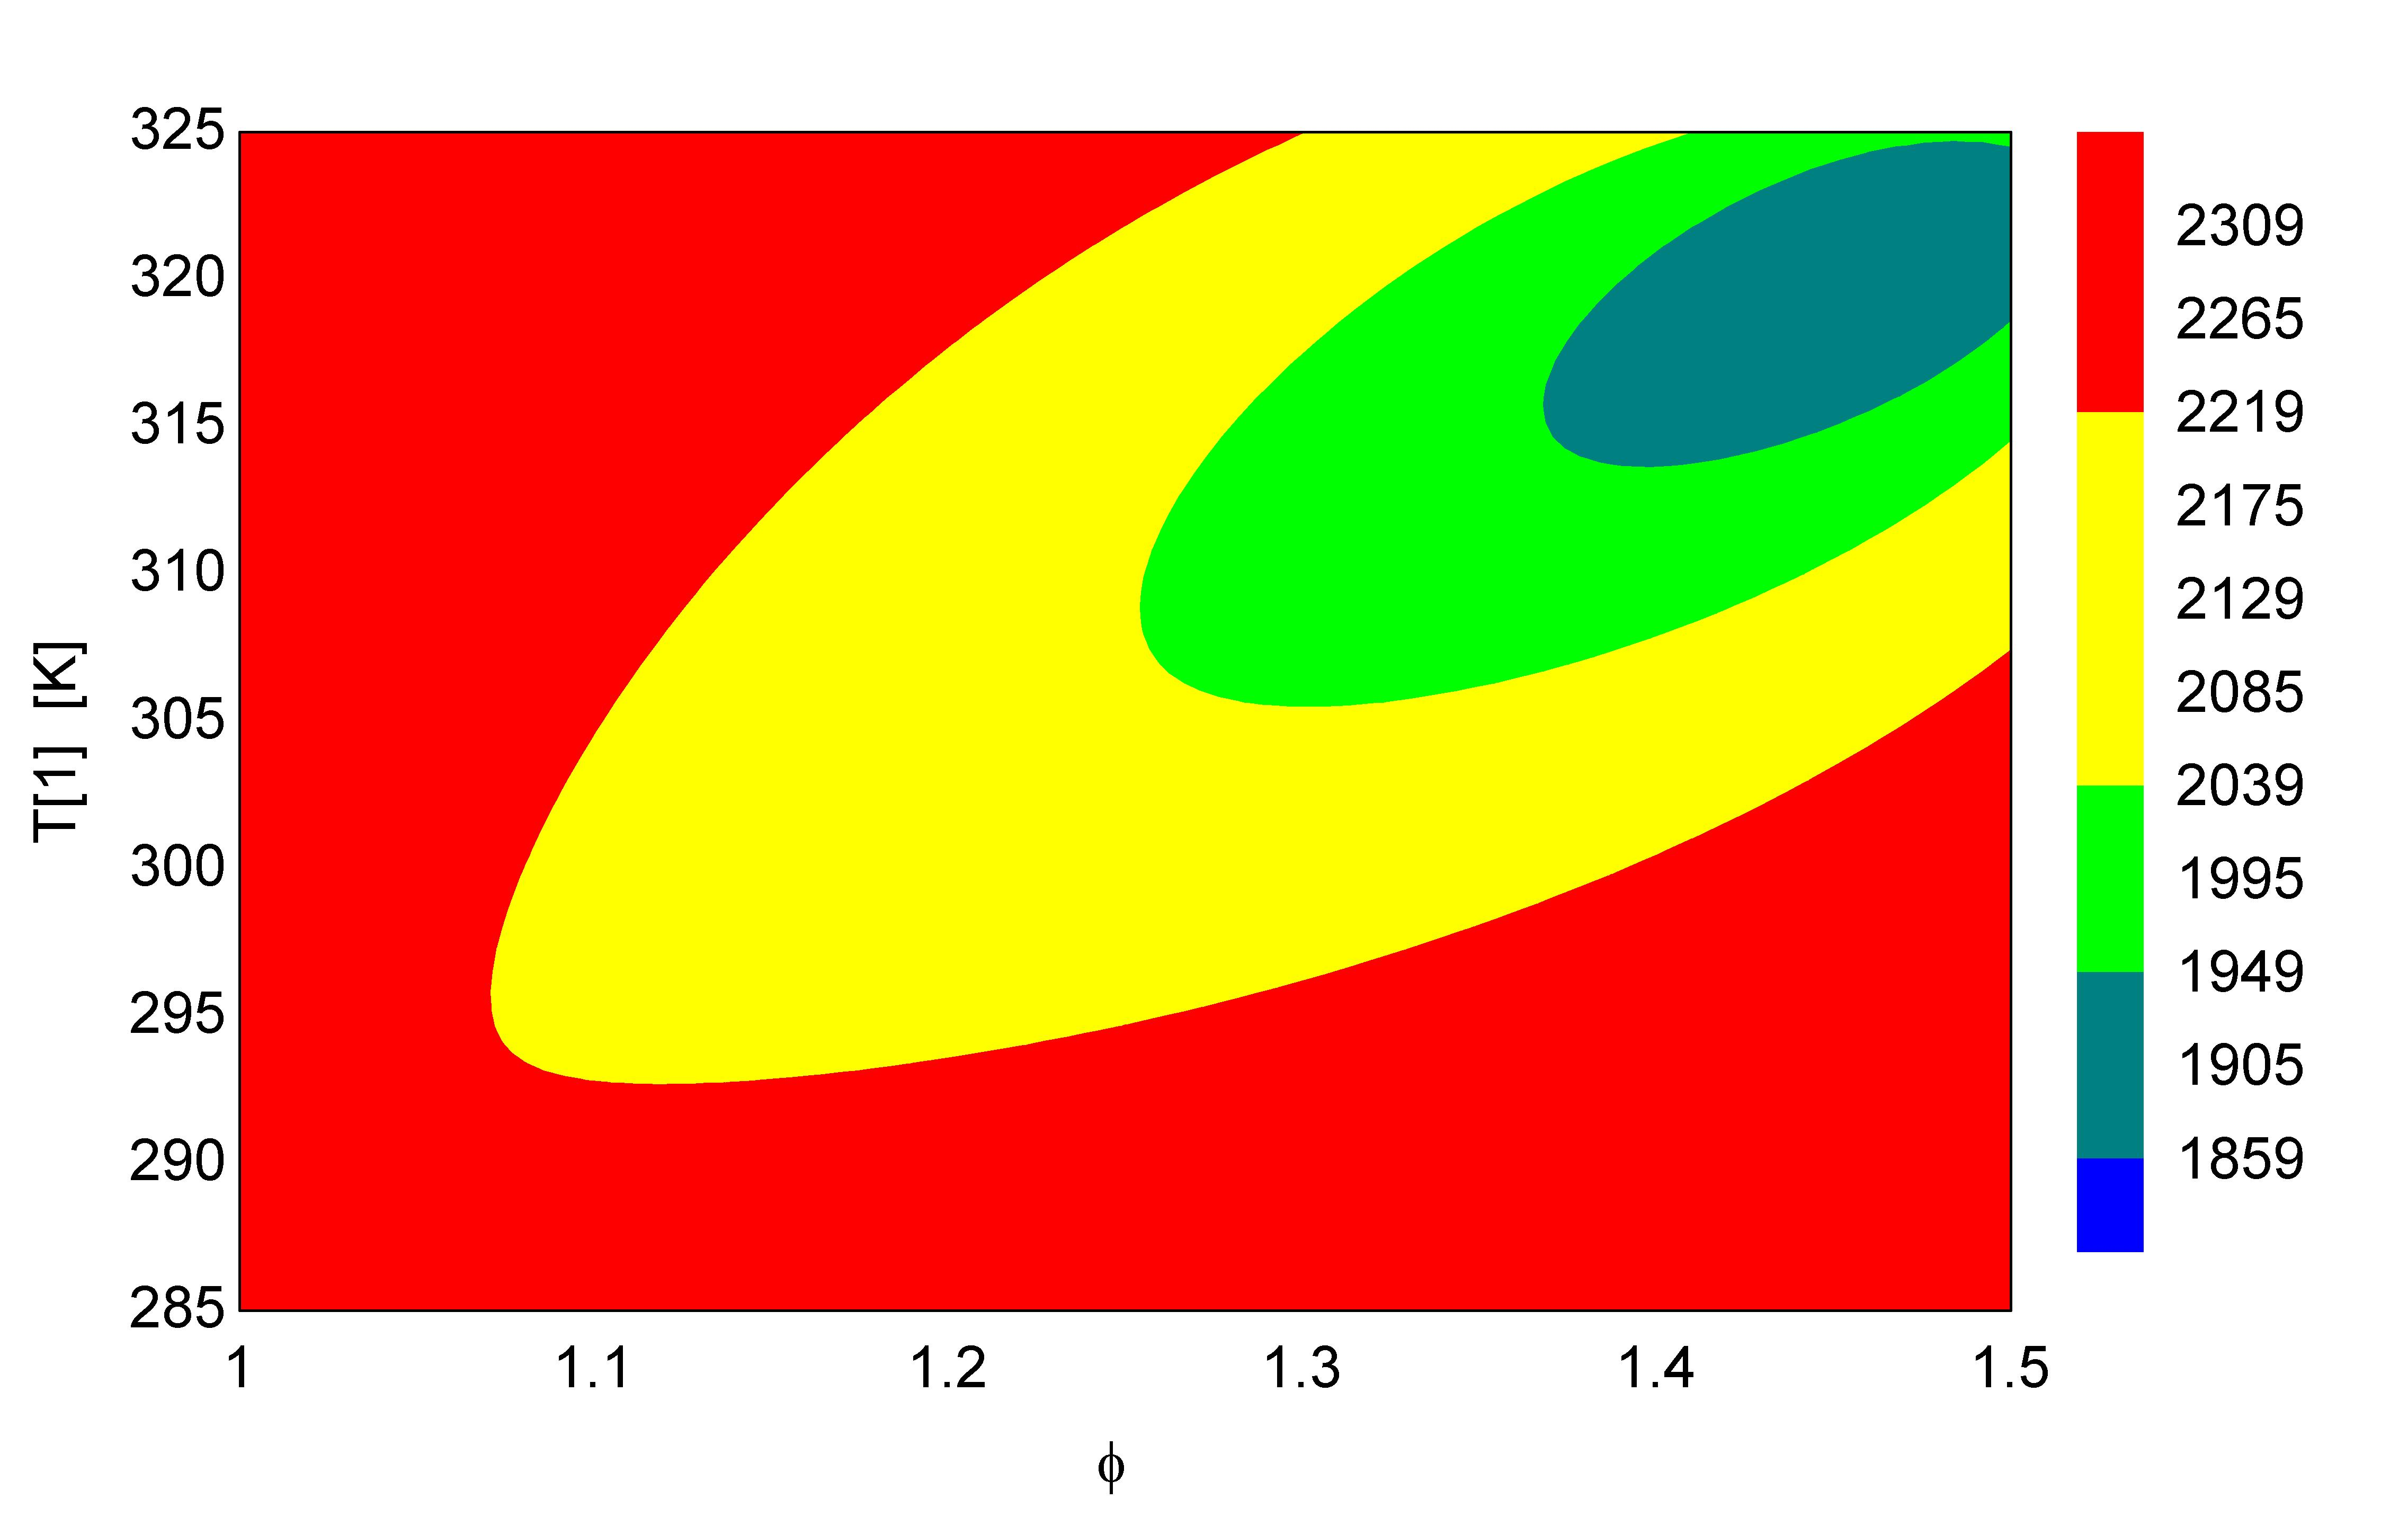
\includegraphics[width=8.0cm,keepaspectratio]{taller1_P1.jpg}}
En la gráfica anterior podemos observar que, a medida que aumenta el exceso de aire, la temperatura de la flama adiabática disminuye. Se aumenta la cantidad de oxígeno disponible, pero también se incrementa la cantidad de nitrógeno y otros gases que no reaccionan en la combustión, por lo que la energía liberada de la combustión deberá distribuirse en un mayor volumen de gases. Por otro lado, la temperatura de la flama adiabática aumenta con la temperatura inicial del aire. Esto se debe a que una mayor temperatura inicial del aire aumenta la energía disponible para la combustión, lo que resulta en una temperatura de flama adiabática más alta.
\subsection*{Plot Window 2:\;ExcessAir\;vs\;T[1]\;vs\;Product N_2}
{\centerline{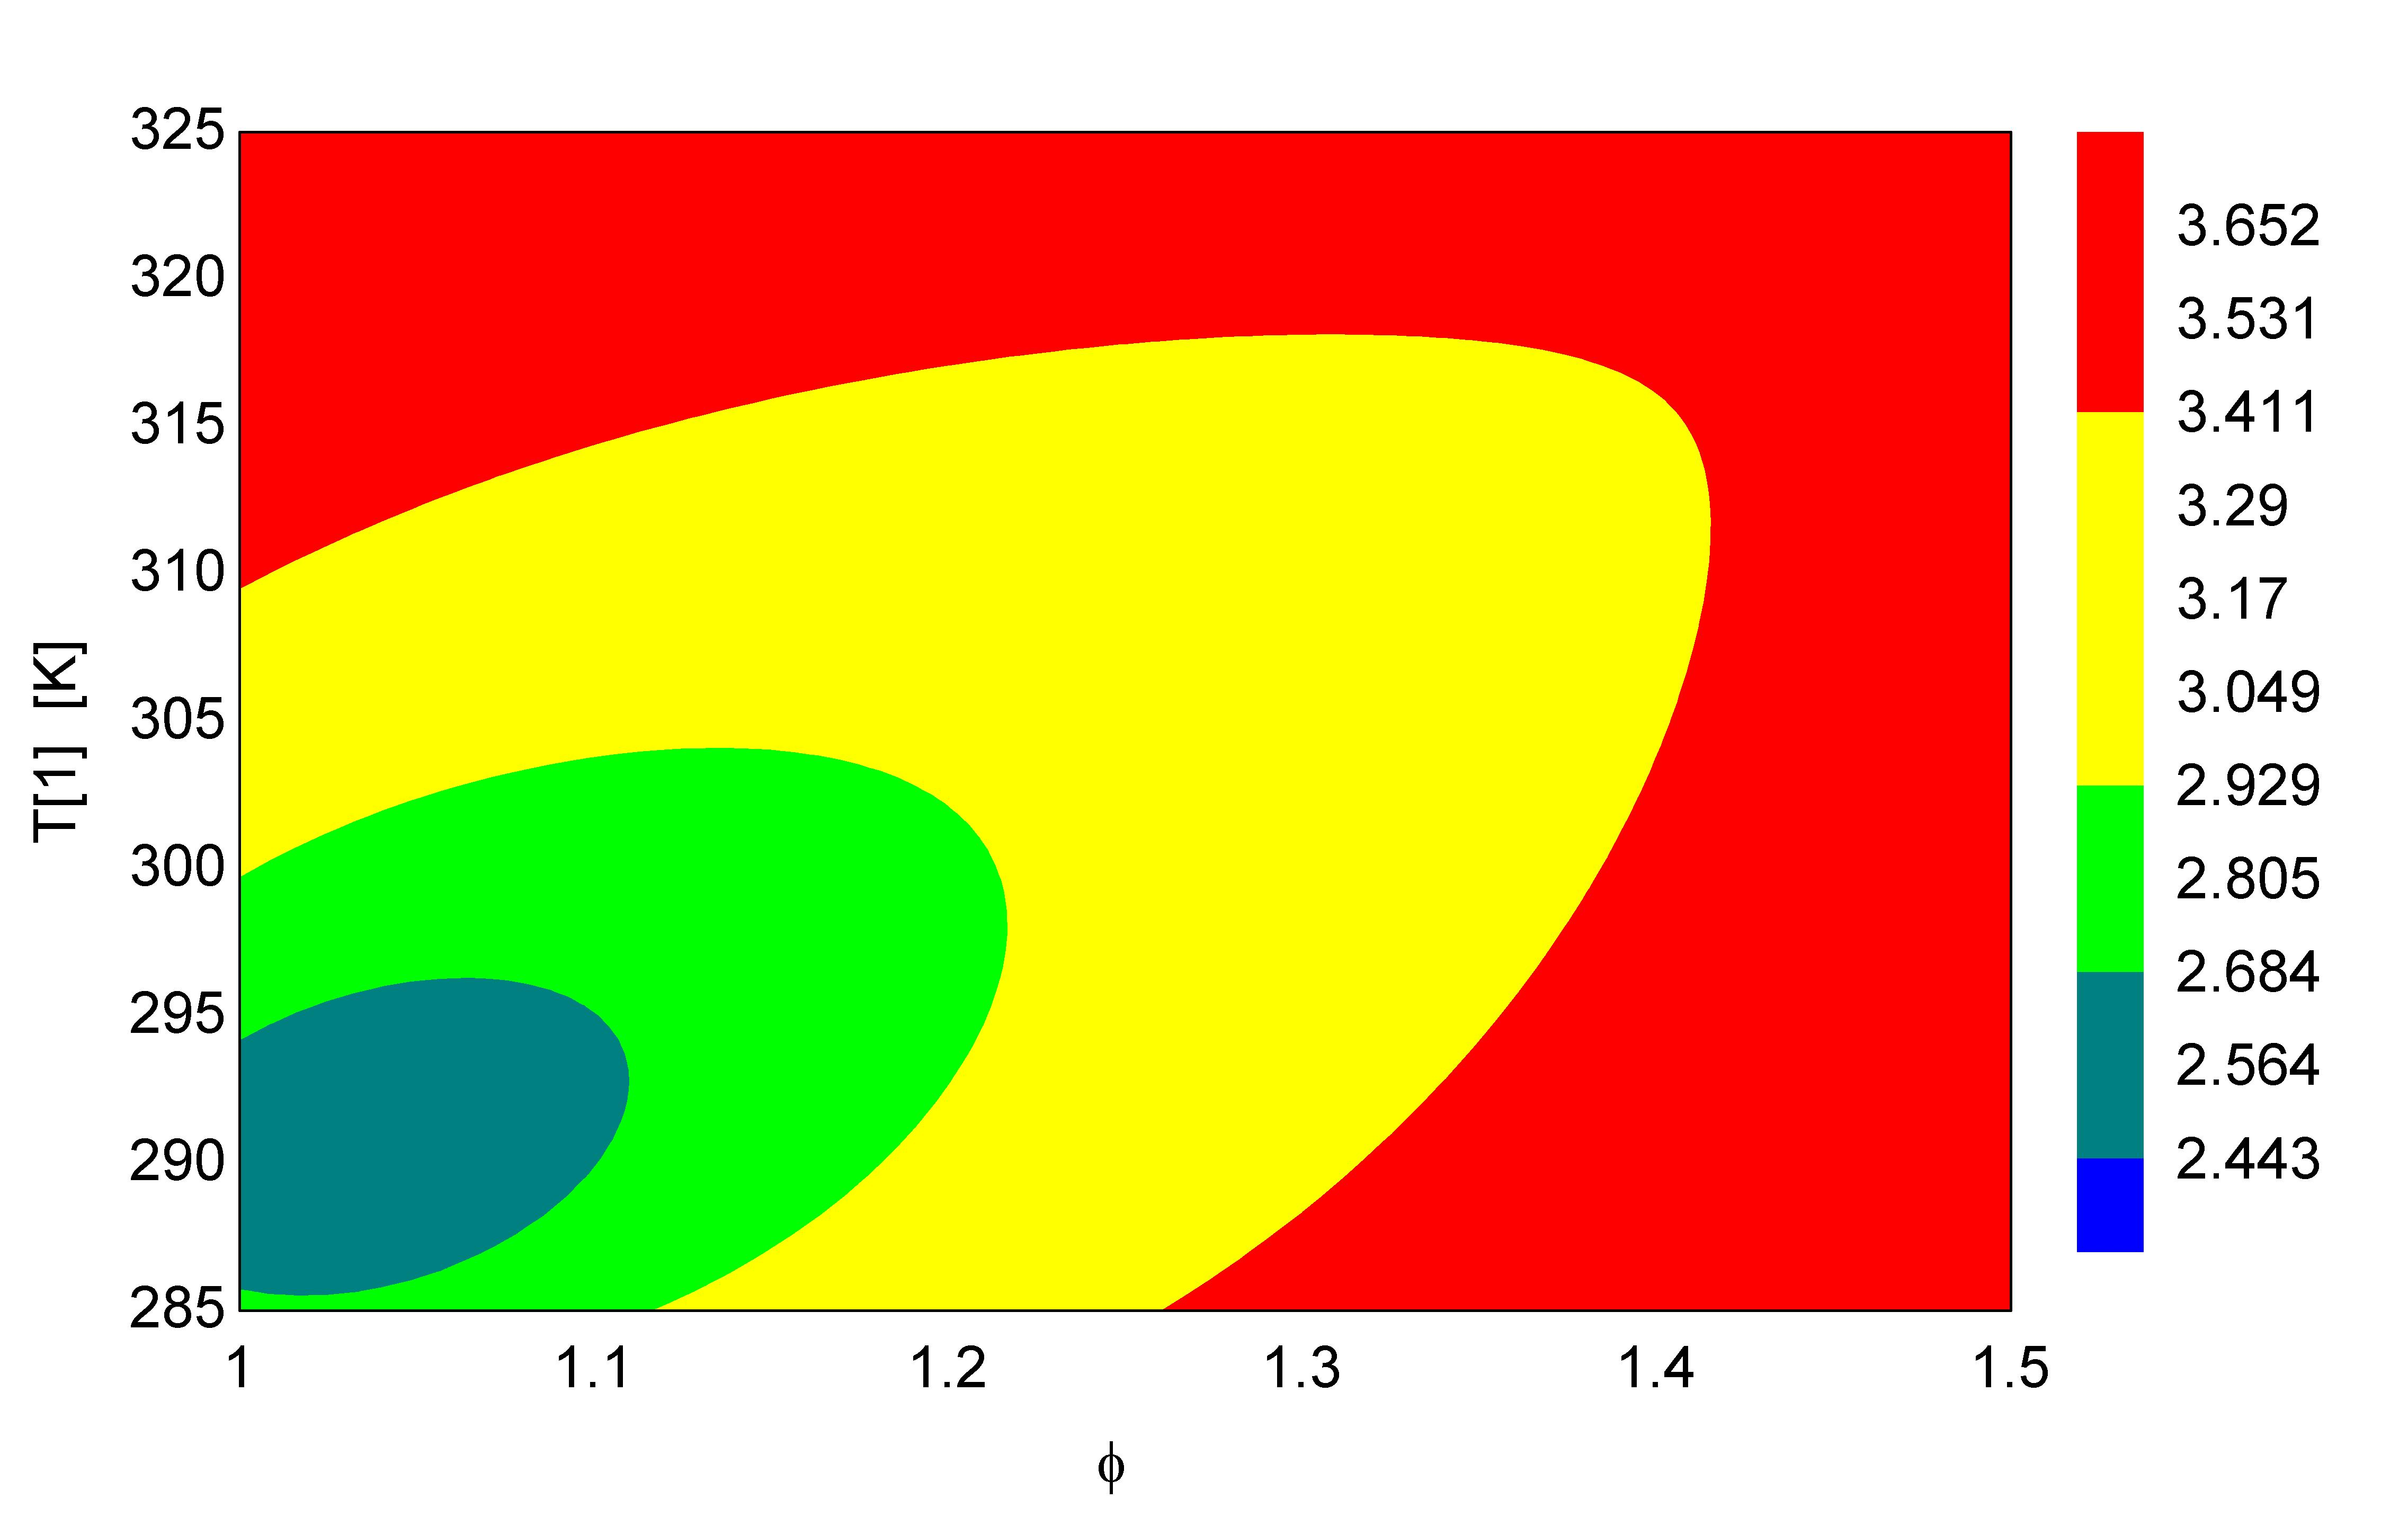
\includegraphics[width=8.0cm,keepaspectratio]{taller1_P2.jpg}}
En la gráfica anterior podemos observar que, a medida que aumenta el exceso de aire, la concentración de nitrógeno en los productos de combustión aumenta. Esto se debe a que el exceso de aire aumenta la cantidad de nitrógeno en los reactivos y por lo tanto en los productos de combustión.
\subsection*{Plot Window 3:\;ExcessAir\;vs\;T[1]\;vs\;Product O_2}
{\centerline{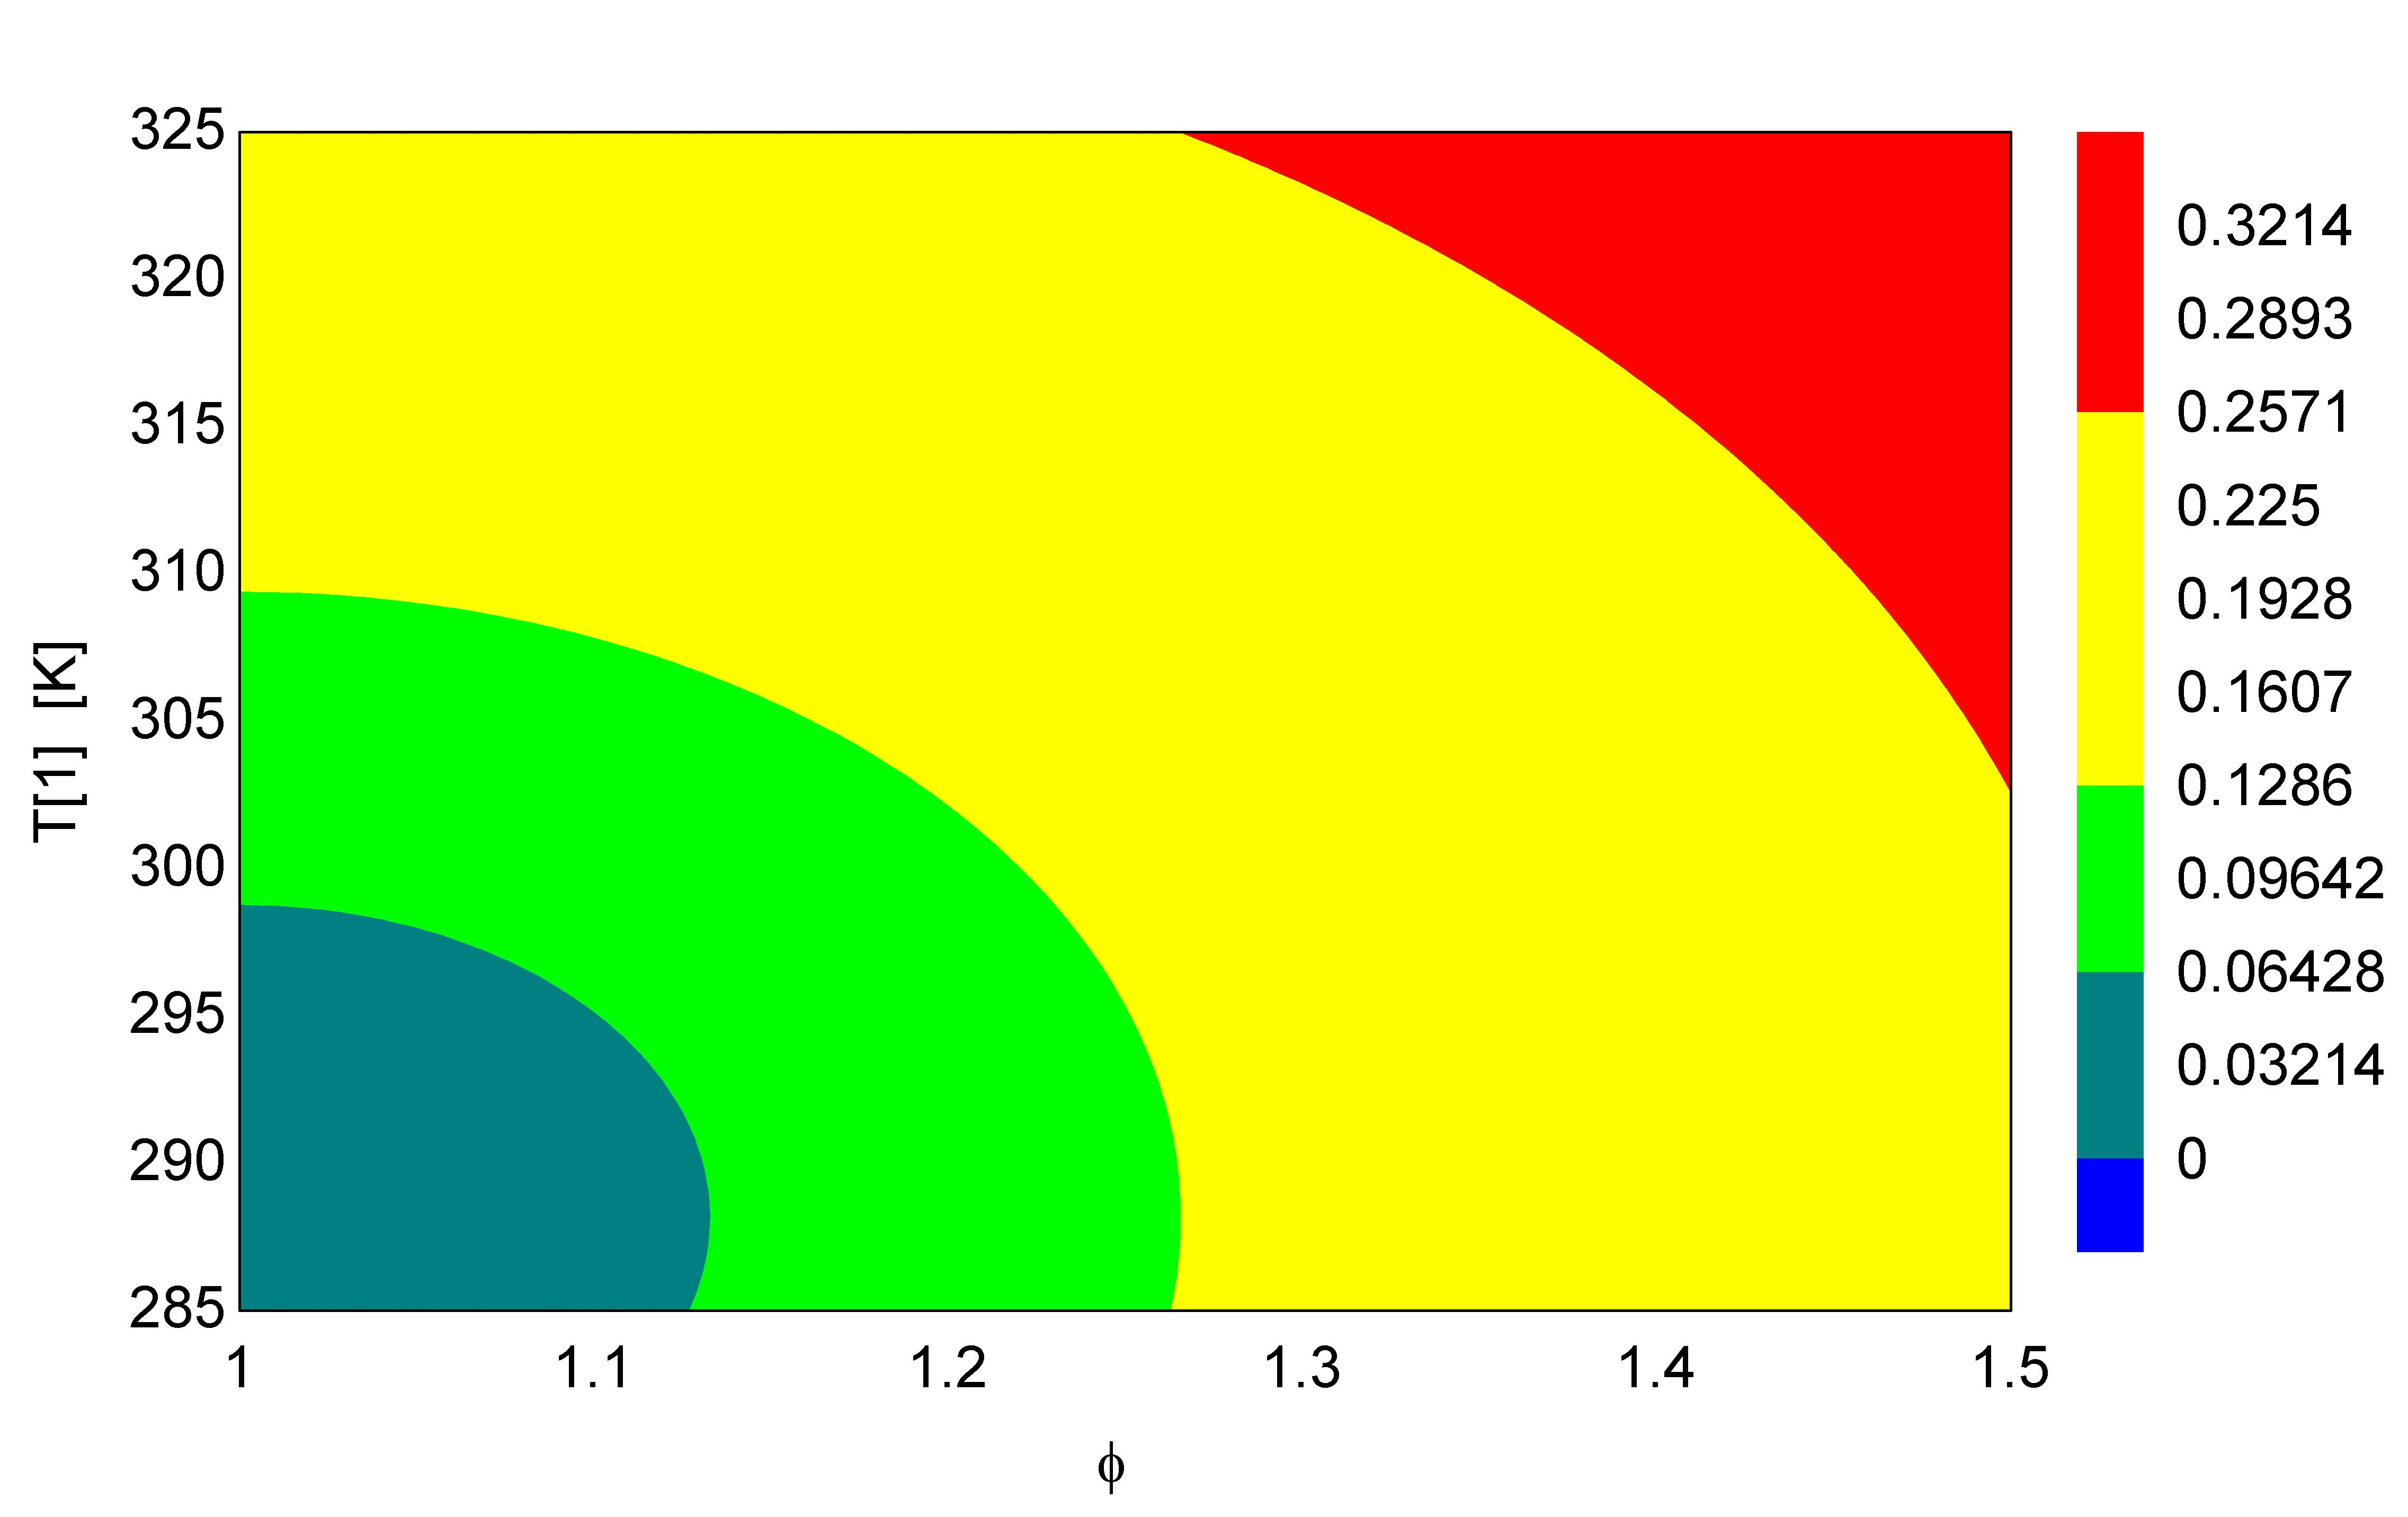
\includegraphics[width=8.0cm,keepaspectratio]{taller1_P3.jpg}}
En la gráfica anterior podemos observar que, análogamente al nitrógeno a medida que aumenta el exceso de aire la concentración de oxígeno en los productos de combustión aumenta. Esto se debe a que el exceso de aire aumenta la cantidad de oxígeno en los reactivos y por lo tanto en los productos de combustión. 

\newpage
\bibliographystyle{apacite}
\nocite{*}
\bibliography{termodi}
\end{document}